\documentclass[12pt]{article} % 
\usepackage{fontspec} %To handle the font named Sans Forgetica
\usepackage{lipsum} %For generating dummy text.
\usepackage{graphicx} %To handle images in the document.
\usepackage{setspace}
\usepackage{xcolor}




% Created by Jamie Cropley
% http://jamie.zone




%Set line spacing here for better readability:
\singlespacing %default value anyway
%\onehalfspacing
%\doublespacing


\setmainfont{[SansForgetica-Regular.otf]} %To load the font named Sans Forgetica
\setmainfont[AutoFakeBold=1.5, AutoFakeSlant=0.4]{[SansForgetica-Regular.otf]}

%\setmainfont{SansForgetica}[
%  Path=./,
%  Extension=.otf,
%  UprightFont=*-Regular,
%  BoldFont=*-Regular,
%  BoldFeatures={FakeBold=3},
%  ItalicFont=*-Regular,
%  ItalicFeatures={FakeSlant=0.3},
%  BoldItalicFont=*-Regular,
%  BoldItalicFeatures={FakeBold=3,FakeSlant=0.3},
%]




\begin{document}


\section*{Title for first paragraph:}
\begin{flushleft}
%Any text I have goes here for one paragraph, in place of lipsum.
\lipsum[1]
\end{flushleft}


\section*{Title for second paragraph:}
\begin{flushleft}
%For a new paragraph write it here in place of lipsum.
\lipsum[1]
\end{flushleft}


%For a new page:
\newpage


\section*{Title for lists:}
\begin{flushleft}
%For lists:
\begin{itemize}
  \item One entry in the list
  \item Another entry in the list
  \begin{itemize}
  \item Sub item example 1
  \item Sub item example 2
  \begin{itemize}
  \item A sub sub item 1
  \item A sub sub item 2
  \end{itemize}
  \end{itemize}
\end{itemize}
\end{flushleft}


%For a new page:
\newpage


\section*{Planet Earth Image Title:}
\begin{flushleft}
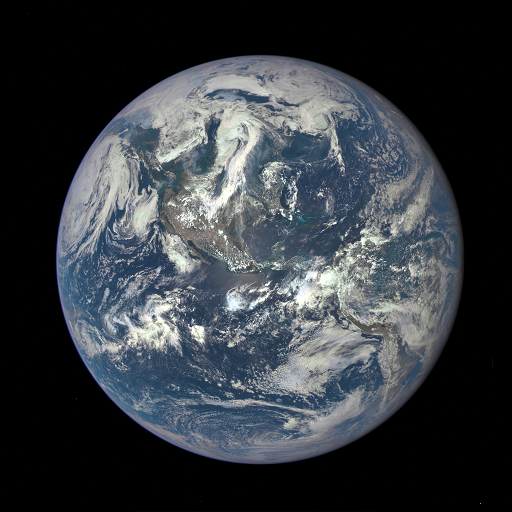
\includegraphics{earth.png} %I can replace this and put any image
\end{flushleft}


%For a new page:
\newpage


\section*{Title for Italic, Bold and Coloured text examples:} %Coloured text can also be applied to section headings.
\begin{flushleft}
\begin{itemize}
\item\textit{Italic text example}
\item\textbf{Bold text example}
\item\textit{\textbf{Bold and Italic text example}}
\item \textcolor{red}{Red text example}
\item \textcolor{green}{Green text example}
\item \textcolor{blue}{Blue text example}
\end{itemize}
\end{flushleft}


% Putting in tabular data: https://www.overleaf.com/learn/latex/Tables


\end{document}